\subsection{Peer Discovery}
\label{sec:p2p:peer-discovery}

Newly connected nodes are lacking information about existing nodes in the network and thus need the help of others to introduce them to the rest of the network. This is done using entry nodes that are announced within the smart contract which creates a Schelling point for new nodes and allows them to connect to other nodes in the network.

By default, each node that joins the network also announces itself within the smart contract. Nodes that chose to act as an entry node, e.g. because they have a public IP address, publish a routable address whilst other nodes solely publish their public key. Thereby, each node receives a list of all nodes that are currently part of the network or have been part it and is thus able to link on-chain events of other nodes, such as opening of payment channels, to off-chain HOPR addresses. Since there is no announcement if a node leaves the network, the list does not provide any information regarding the nodes' availability.

Apart from the smart contract, all nodes in the network share addresses of each other in a Kademlia \cite{kademlia} distributed hash table (DHT). Once a node has established a connection to one of the entry nodes, it connects to the DHT and publishes additional addresses, see figure \ref{fig:address-announcement}. This includes first of all relay addresses since they are subject of change due to the availability of the utilized relay nodes, as well as additional direct addresses that help nodes to connect to other nodes running in the same local network or on the same machine.

\begin{figure}[H]
    \centering

    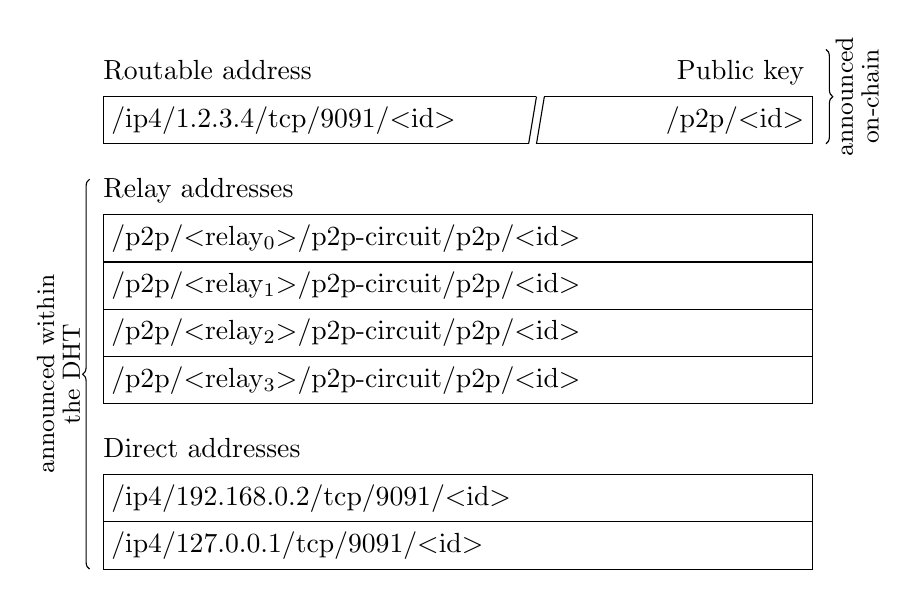
\begin{tikzpicture}
        \def\one{0.6}
        \def\nodeWidth{9}
        \def\nodeWidthMinusPadding{8.8}
        \def\nodeHeight{\one}
        \def\padding{0.1}
        \def\numberOfRelays{3} % +1
        \def\nodeOffset{1}

        % Routable address
        \path (0,0) rectangle (\nodeWidth,\nodeHeight) node [midway,text width=\nodeWidth cm] {\strut{}Routable address};

        \begin{scope}[shift={(0,-0.6)}]
            \draw (\nodeWidth/2+\nodeOffset,\nodeHeight) -- (0,\nodeHeight) -- (0,0) -- (\nodeWidth/2+\nodeOffset-\padding,0);
            \draw (\nodeWidth/2+\nodeOffset+\padding,\nodeHeight) -- (\nodeWidth,\nodeHeight) -- (\nodeWidth,0) -- (\nodeWidth/2+\nodeOffset,0);
        \end{scope}
        \path (0,0) rectangle (\nodeWidth,\nodeHeight) node [midway,text width=\nodeWidthMinusPadding cm,align=right] {\strut{}Public key};
        \path[shift={(0,-0.6)}] (0,0) rectangle (\nodeWidth,\nodeHeight) node[midway,text width=\nodeWidthMinusPadding cm] {/ip4/1.2.3.4/tcp/9091/\textless{}id\textgreater{}} node[midway,text width=\nodeWidthMinusPadding cm,align=right] {/p2p/\textless{}id\textgreater{}};

        \draw (\nodeWidth/2+\nodeOffset,0) -- (\nodeWidth/2+\nodeOffset-\padding,-\nodeHeight);
        \draw (\nodeWidth/2+\nodeOffset+\padding,0) -- (\nodeWidth/2+\nodeOffset,-\nodeHeight);

        % Relay addresses
        \begin{scope}[shift={(0,-1.5)}]
            \path (0,0) rectangle (\nodeWidth,\nodeHeight) node [midway,text width=\nodeWidth cm] {\strut{}Relay addresses};

            \foreach \i in{0,...,\numberOfRelays} {
                    \draw[shift={(0,-\one-\i*\one)}] (0,0) rectangle (\nodeWidth,\nodeHeight) node[midway,text width=\nodeWidthMinusPadding cm] {/p2p/\textless{}relay$_\i$\textgreater{}/p2p-circuit/p2p/\textless{}id\textgreater{}};
                }
        \end{scope}

        % Direct addresses
        \begin{scope}[shift={(0,-3.0-\one*\numberOfRelays)}]
            \path (0,0) rectangle (\nodeWidth,\nodeHeight) node [midway,text width=\nodeWidth cm] {\strut{}Direct addresses};

            \draw[shift={(0,-\one)}] (0,0) rectangle (\nodeWidth,\nodeHeight) node[midway,text width=\nodeWidthMinusPadding cm] {/ip4/192.168.0.2/tcp/9091/\textless{}id\textgreater{}};
            \draw[shift={(0,-2*\one)}] (0,0) rectangle (\nodeWidth,\nodeHeight) node[midway,text width=\nodeWidthMinusPadding cm] {/ip4/127.0.0.1/tcp/9091/\textless{}id\textgreater{}};
        \end{scope}

        \draw[decoration={brace,raise=5pt,mirror},decorate] (0,-1.05) -- node[left=5pt] {\rotatebox{90}{\small{\shortstack{announced within\\the DHT}}}} (0,-4.2-\one*\numberOfRelays);

        \draw[decoration={brace,raise=5pt},decorate] (\nodeWidth,0.6) -- node[right=5pt] {\rotatebox{90}{\small{\shortstack{announced\\on-chain}}}} (\nodeWidth,-0.6);
    \end{tikzpicture}
    \caption{Address announcment within the HOPR network.}
    \label{fig:address-announcement}
\end{figure}

Apart from the altruistic benefit to the network when announcing as an entry node, it is expected that the announcement does not immediately lead to payout. Nevertheless, since the \lcnameref{sec:path-selection} mechanism prefers nodes with higher availability, it is that well-known entry nodes with a good availability are chosen more likely as a relayer which thus increases their rewards on a longer term.

Using announcments on a public blockchain comes with the property that a potential adversary who attempts to run an eclipse attack against a newly connected node also needs to provide a sound and fake blockchain which is assumed to be hard. Hence, the attacker is unable to withhold entry nodes but nevertheless, but it is able to spam the victim with connection information about collaborating nodes.